\section{Project Management}\label{management} 
    In this section, we'll take look at how we organized the team, a brief risk assesment, and an evaluation of the work process. 
    
    \subsection{Team Organization}\label{team} 
        [The team structure and roles.]
        
        This section describes in detail how we organize ourselves and how we split roles and tasks among the team members. We have a flat team structure and have shifted our focus accordingly over to team communication. 
    
    \subsubsection{Team Structure}
    We already know each other coming into the project so we have chosen a flat organisational structure, since all decisions within the team will more or less be made by all the members together either way. Relying on the entire group for decisions will both involve and invest everyone in the project and will work well with our already existing group dynamic.
    \footnote{
        Flat organization structure is a structure with few or no levels of intervening management. The idea is that well-trained workers will be more productive when they are directly involved with decision making. 
        \href{http://en.wikipedia.org/wiki/Flat_organization}{Wikipedia: Flat Ogranization Structure} 
    }
    
    \begin{figure}[h]
        \centering
        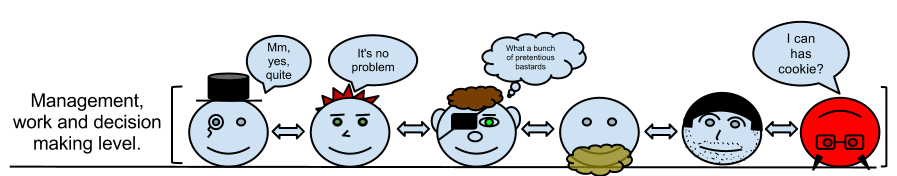
\includegraphics[scale=0.5]{TeamOrganizationchart}
        \caption{Team Organization chart}
        It was made during lunch, but the general principle still remains, that the structure is flat.
        \label{fig:teamOrgchart}
    \end{figure}
    
    %Why changing roles does not work in our structure and how we solve the challenges that might occur in this association. 
    As the structure is shown in the chart. There is no difference in what responsibility level anyone have, or what role one has. The concept of changing roles weekly is good for a learning situation but very inefficient where knowledge and research are key components in a limited timed project like this. We anticipate that the time for this project probably won't be sufficient. And therefore we have to keep people focused on the task they have taken, while they have the current research fresh in mind and can continue the current progress. If we were to change the tasks/roles every week, the newly assigned person would waste time learning existing knowledge at the beginning of every week.

    We chose to drop responsibility areas and roles. Instead we look at tasks. We might have tasks representing a responsibility, but it is still a task with a person assigned to the task. This makes the team more flexible. We don't run the risk of a key member of our team becoming ill and the rest of the group don't have a clue as to whats left to do on that particular responsibility area. Instead we say: "that person is ill, and we have to do this task by Monday then I'll do it". And the task gets done.
    
    The problem we encounter and discharge is the eventuality of a person becoming ill or incapacitated and at the same time having key knowledge to our project. This seemingly huge problem is not really a problem as we document a lot. So the knowledge of a person is at all times documented, to such a degree that if a person is incapacitated the other team members can pick up right where he left off, thereby expelling the problem altogether. 
    
    Further, the team structure and the lack of responsibility areas gives us the chance to define how we want to deal with task and their priority. The work flow that we have makes us prioritise tasks continuously and get the most pressing task done at any give time. It's similar to a max heap. We put tasks in to the heap, heapify(prioritise tasks) and choose(pop) the maximized task, the task that has the highest priority. 
    
    %Task division and delegation.
    When we assign task to people we consider the persons interest, experience and existing knowledge. Most times the tasks fall naturally to one person that has worked with similar tasks earlier in the project. Other times there is more of lottery, where the task has no prerequisites. Then we choose an available person often volunteering for the task, or we easily delegate them with a question, "Can you do that?". Task delegation and sharing the work load has not been a problem during the project.
    
    %benefits of a flat team structure.
    
    
    \subsubsection {Team communication}
    We will work together from 10 to 16, Monday through Thursday every week, with allowed exceptions for lectures and such. Group members can also work in their free time to make up for missed collaboration hours or to just put in some extra work. This means more work than the course requires, but we decided that we want to do it this way so we can either take some time off now and then, or have more time for the exams in May.

    The customer has not given us many strict requirements, but instead they have suggested a few things that we could do. Given this freedom, we decided that we should improve on the base requirements by adding most of the things mentioned in this section.
    
    We will not be able to have frequent face to face meetings with the customer, but we will have weekly online meetings with them instead, as well as e-mail communication as needed. Since we have seen what happens in projects where there is little to no communication, we decided, in agreement with the costumer, that we at least wanted to have weekly meetings in order to keep a good dialog with the customer, and also give them the opportunity to take part in the development of the project. Since we have some challenges in the fact that the customer is in Oslo, we decided that the weekly meetings will be held over Skype.
    
    \subsection{Risk Assesment}\label{risk}
    
    \subsection{Process Evaluation}\label{processevaluation}
    % Write something about the fact that we use one day a week to work with planning and paperwork. 
    

